\section{Background}
This section will contain the relevant background. Consider the following items:
\begin{itemize}
\item Application specific processor
\item Non-Volatile Memories
\item Static Data-Dependency Analysis
\item System Under Analysis
\end{itemize}

\subsection{System Under Analysis}
\label{ssec:system_under_analysis}
The system architecture we use in this work is composed of two levels of memory and a \textit{Custom Processor}. Taking advantage of the possibility to produce stacked chip having levels produced using different manifacturing technologies we are able to explore different memory implementations at the \textit{Level 2} of the memory architecture. The first layer of memory - \textit{Level 1} - is instead fabricated on the same chip layer as the Custom Processor and uses SRAMs memories. The diagram in Figure~\ref{fig:system} shows a representation of the entire computing system.
The computation proceed as described in Figure~\ref{fig:system}. At the beginning of the computation we assume that all of the required input data are present at the \textit{Level 2} of the memory hierarchy. In the first stage of the computation the input data are transfered to the \textit{Custom Processor} using the \textit{Level 1} memory as intermediate storage location. The actual computation is peformed in the second stage where each output element is stored in the \textit{Level 1} memory. Once the computation is compleate, in the third step, the output data stored in the \textit{Level 1} memory is transfered to the \textit{Level 2} memory. At the end of the three stages of the computation the result will be stored in the \textit{Level 2} memory.

\begin{figure}[tb] 
\centering
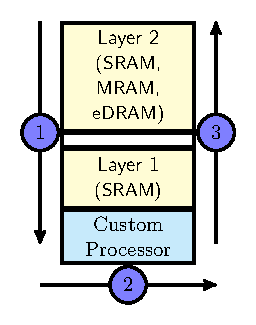
\includegraphics[width=0.25\columnwidth]{images/architecture.pdf}
\caption{\small The system under analysis. Composed by two levels of memory, the memory at layer two can use various technologies while the memory at layer one uses only SRAM technology.}
\label{fig:system}
\end{figure}

\subsection{Level 2 Memory Model}
\label{ssec:layer2_model}
We model the \textit{Level 2} memory as accessible using burst accesses. 
%Figure~\ref{fig:l2model}  shows a representation of such access. 
A read or write access to the \textit{Level 2} memory is controlled by a Direct Memory Access (DMA) controller. Starting address and size of the burst are given as input to the DMA, which perform the burst memory access. After an initial setup time the accessed elements are transfered in sequence from the starting address to the ending address to the \textit{Level 1} memory if a read access is being berformed, or to the \textit{Level 2} memory if a write access is being performed.

%\begin{figure}[tb] 
%\centering
%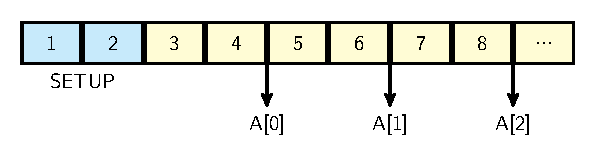
\includegraphics[width=\columnwidth]{images/l2_model.pdf}
%\caption{\small Example of Level 2 memory burst access.}
%\label{fig:l2model}
%\end{figure}
